\documentclass[12pt]{article}

% Idioma e codificação
\usepackage[brazil]{babel}
\usepackage[utf8]{inputenc}
\usepackage[T1]{fontenc}

% Matemática e listas
\usepackage{amsmath, amssymb, amsfonts}
\usepackage{enumitem}

% Layout e cores
\usepackage{geometry}
\usepackage{graphicx}
\usepackage{xcolor}
\usepackage{listings}
\usepackage{hyperref}

% Cores institucionais
\definecolor{maincolor}{RGB}{0,100,50}
\definecolor{forestgreen}{RGB}{0,100,50}

% Cabeçalho e rodapé
\usepackage{fancyhdr}

% Blocos
\usepackage[most]{tcolorbox}
\newtcolorbox{block}[1]{%
  colback=green!5,
  colframe=maincolor,
  coltitle=white,
  title=#1,
  fonttitle=\bfseries,
  boxrule=1.5pt,
  arc=3mm,
  left=6pt,
  right=6pt,
  top=6pt,
  bottom=6pt
}

% Margens
\geometry{margin=2.5cm}

% Fancyhdr
\pagestyle{fancy}
\fancyhf{}

\renewcommand{\headrulewidth}{2pt}
\renewcommand{\footrulewidth}{2pt}

\renewcommand{\headrule}{\hbox to\headwidth{%
  \color{forestgreen}\leaders\hrule height \headrulewidth\hfill}}

\renewcommand{\footrule}{\hbox to\headwidth{%
  \color{forestgreen}\leaders\hrule height \footrulewidth\hfill}}

\setlength{\headheight}{52pt}
\addtolength{\topmargin}{-20pt}

\fancyhead[L]{%
  
\includegraphics[height=1.2cm]{Universidade_de_Rio_Verde.jpg}
}

\fancyhead[R]{%
  \raggedleft
  \textcolor{forestgreen}{%
    \small
    \textbf{Atividade Prática: Manipulação de Dados com SQL}\\
    Me.~Sergio Souza Novak\\
    \textit{Banco de Dados I}
    }
    }

\fancyfoot[C]{\textcolor{forestgreen}{\thepage}}

% Caixa de resposta
\newtcolorbox{resposta}[1]{%
  colback=white,
  colframe=forestgreen!30,
  arc=1mm,
  height=#1,
  width=\textwidth,
  boxrule=0.8pt
}

% Configuração para blocos de código SQL
\lstset{
    language=SQL,
    basicstyle=\ttfamily\small,
    keywordstyle=\color{blue},
    commentstyle=\color{gray},
    stringstyle=\color{orange},
    breaklines=true,
    frame=single,
    rulecolor=\color{black},
    numbers=left,
    numberstyle=\tiny\color{gray},
    showstringspaces=false
}

% =========================
\begin{document}
% =========================

\vspace*{0.2cm}

\begin{center}
  {\Large \textbf{Atividade Prática: Manipulação de Dados com SQL e PostgreSQL}}\\[0.2cm]
  \textit{Instruções: Utilize o pgAdmin 4 para realizar a criação de tabelas, importação de dados externos (CSV) e execução de consultas analíticas.}
\end{center}

\vspace{0.4cm}

\begin{block}{Objetivo da Atividade}
O objetivo desta atividade é realizar a criação de tabelas, importação de dados externos (CSV) e execução de consultas analíticas e de filtragem utilizando o \textbf{pgAdmin 4}.
\end{block}

\vspace{0.5cm}
  
\section*{Estrutura do Conjunto de Dados}

Para esta atividade, utilizaremos um conjunto de dados de imagens de peixes processadas para extração de características. A estrutura de diretórios do projeto é a seguinte:

\begin{verbatim}
.
+-- aplicacao_das_mascaras
|   +-- fish1799.jpg
+-- bd
|   +-- fish1799.jpg
+-- bd_mask
|   +-- fish1799.jpg
+-- dados_analytics
    +-- df_final_integrado.csv
\end{verbatim}

\begin{itemize}
    \item \textbf{bd/}: Contém as imagens originais dos peixes capturadas em ambiente controlado.
    \item \textbf{bd\_mask/}: Contém as máscaras binárias (preto e branco) resultantes do processo de segmentação, onde o peixe é isolado do fundo.
    \item \textbf{aplicacao\_das\_mascaras/}: Resultado da aplicação da máscara sobre a imagem original, removendo completamente o ruído do fundo.
    \item \textbf{dados\_analytics/}: O arquivo \texttt{df\_final\_integrado.csv} contém as métricas extraídas que serão importadas para o banco de dados.
\end{itemize}

\subsection*{Atributos do Arquivo CSV}

O arquivo \texttt{df\_final\_integrado.csv} possui as seguintes colunas (atributos):

\begin{description}
    \item[id:] Nome do arquivo da imagem original (ex: \texttt{peixe\_180.jpg}).
    \item[area:] Número total de pixels que compõem a silhueta do peixe.
    \item[perimetro:] Comprimento da borda externa da silhueta.
    \item[ecentricidade:] Medida de "alongamento" da forma (0 para um círculo, próximo de 1 para uma linha).
    \item[maior\_eixo:] Comprimento do maior diâmetro da elipse que circunda o peixe.
    \item[menor\_eixo:] Comprimento do menor diâmetro da elipse que circunda o peixe.
    \item[peso:] Peso real do peixe em gramas (utilizado para supervisão/treinamento).
    \item[classe:] Faixa de peso do peixe.
    \item[compactacao:] Razão entre a área e o quadrado do perímetro (indica a "redondeza").
    \item[Rmm:] Razão entre o maior eixo e o menor eixo.
    \item[centroid\_x / centroid\_y:] Coordenadas do centro de massa do peixe na imagem.
\end{description}

\begin{figure}[h]
    \centering
    \begin{minipage}{0.31\textwidth}
        \centering
        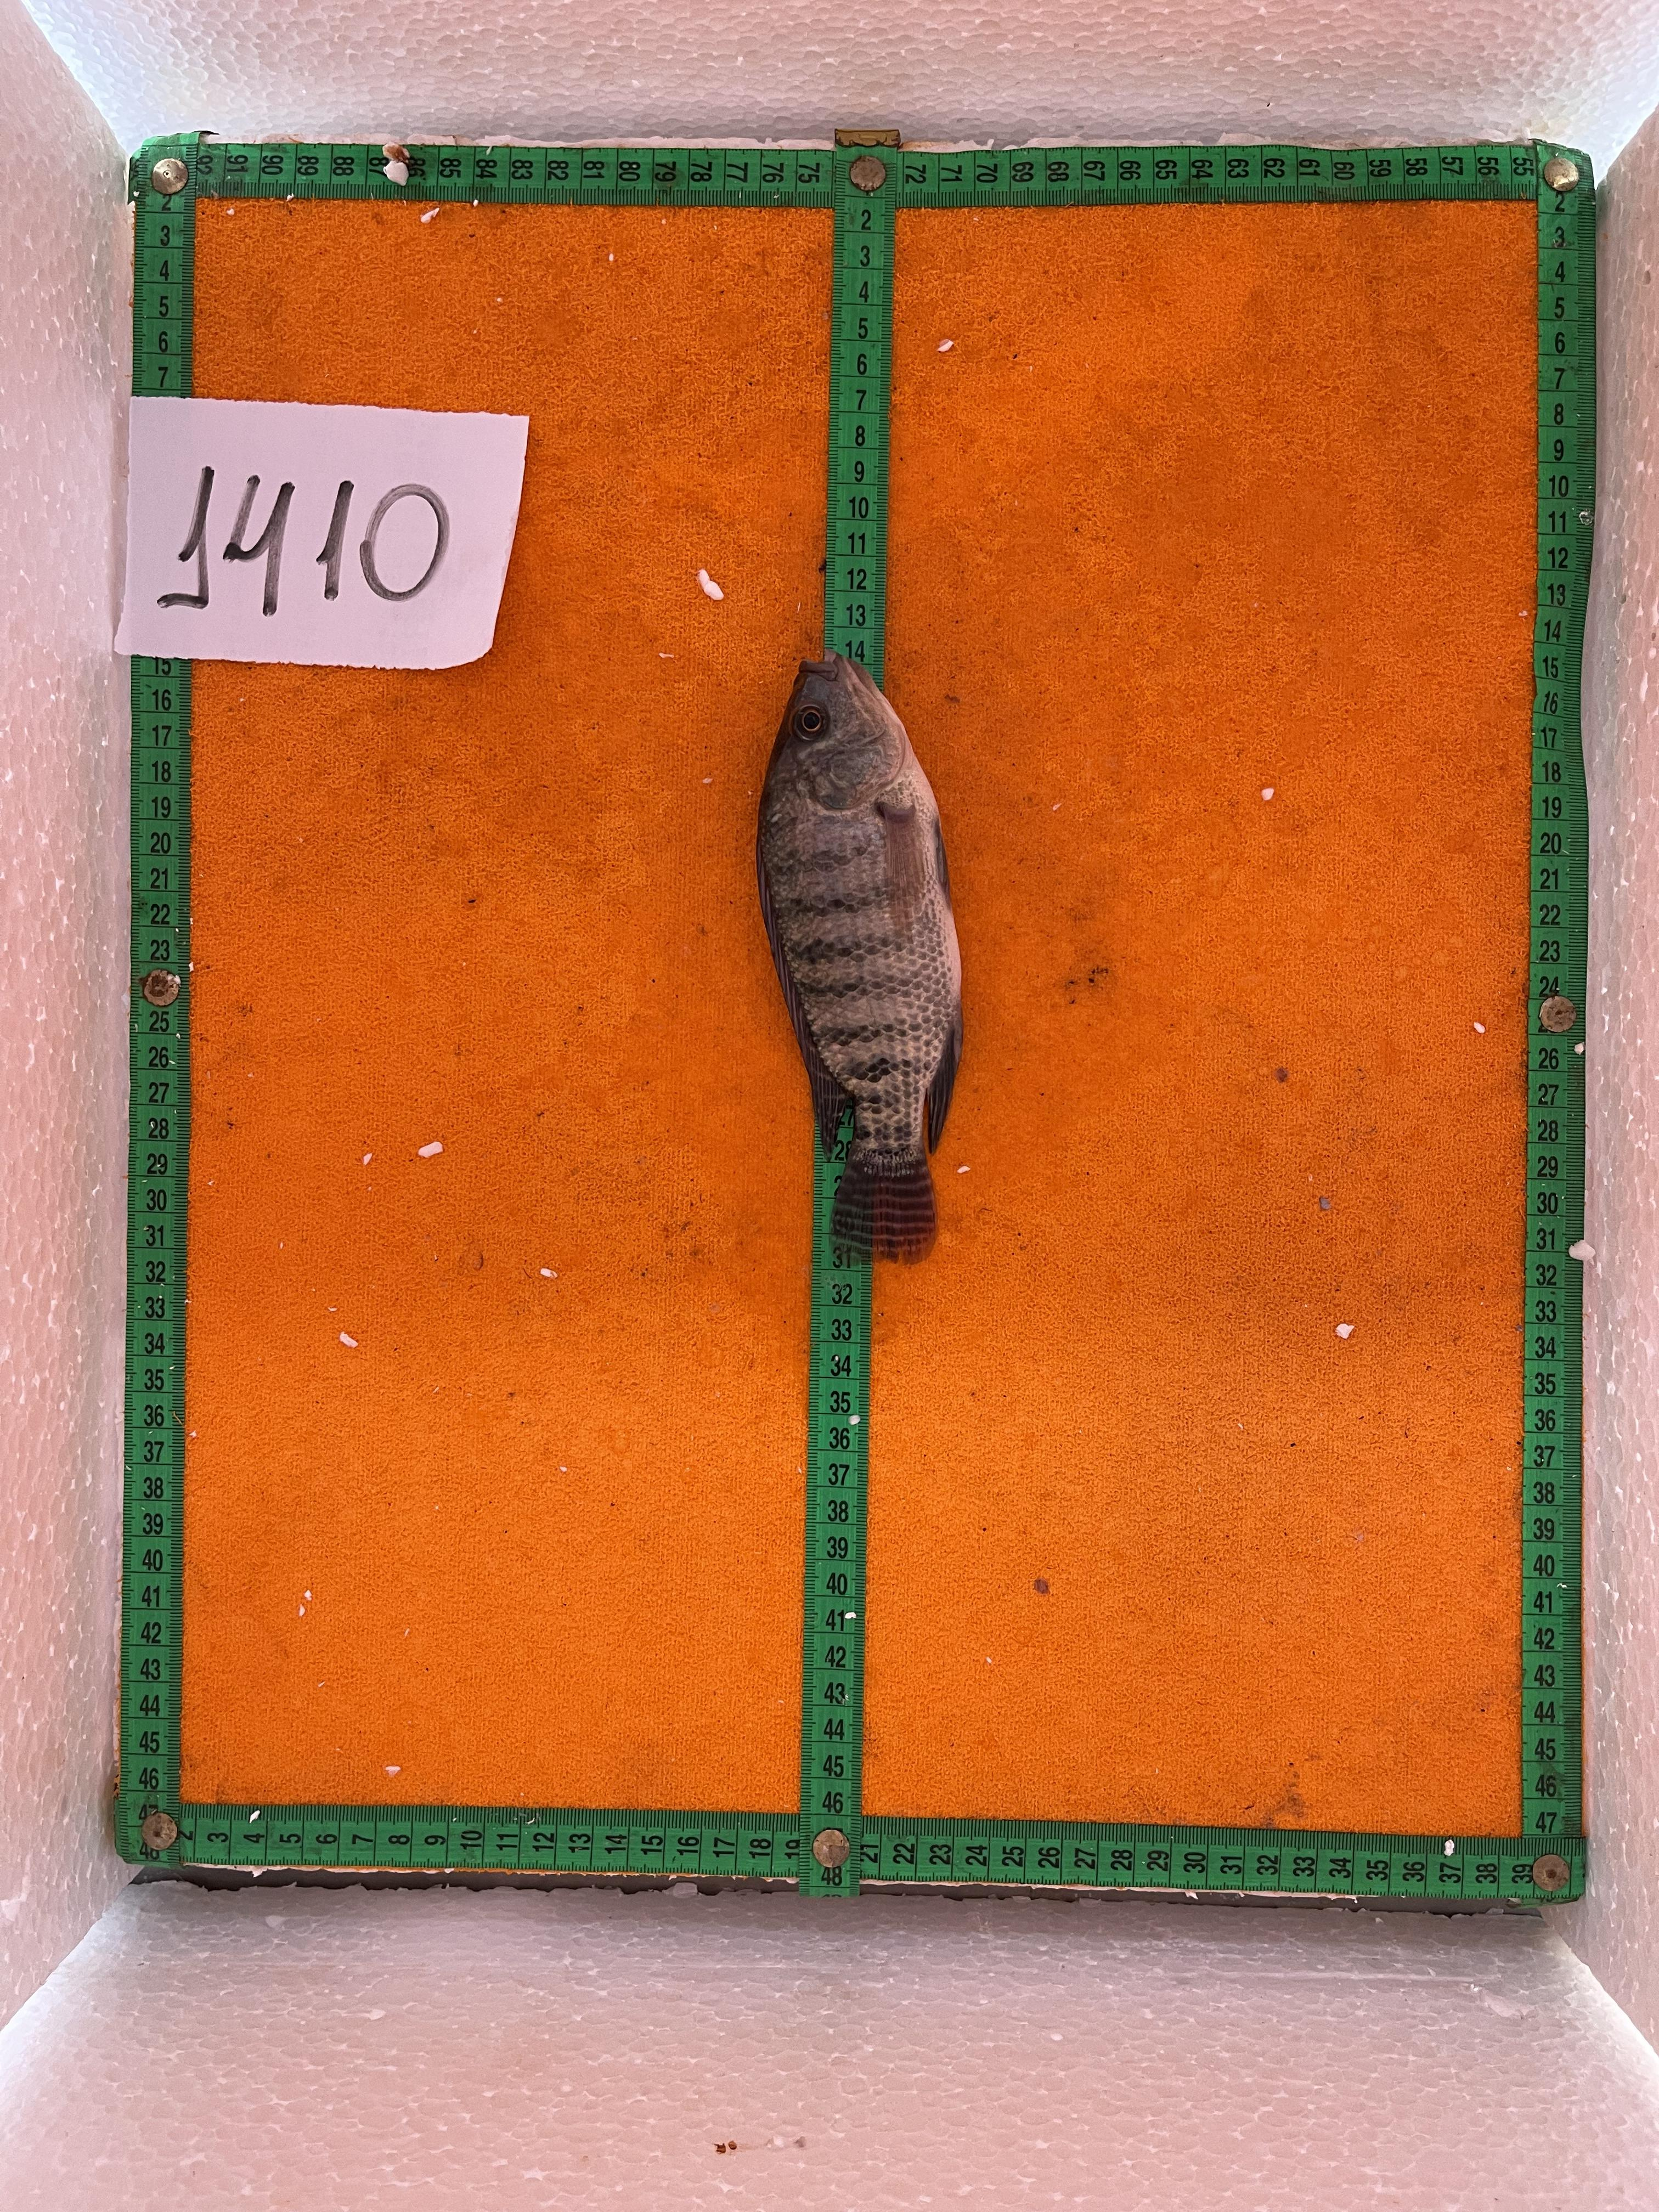
\includegraphics[width=\textwidth]{base_pesos_peixe/bd/fish1799.jpg}
        \caption*{Original}
    \end{minipage}
    \hfill
    \begin{minipage}{0.31\textwidth}
        \centering
        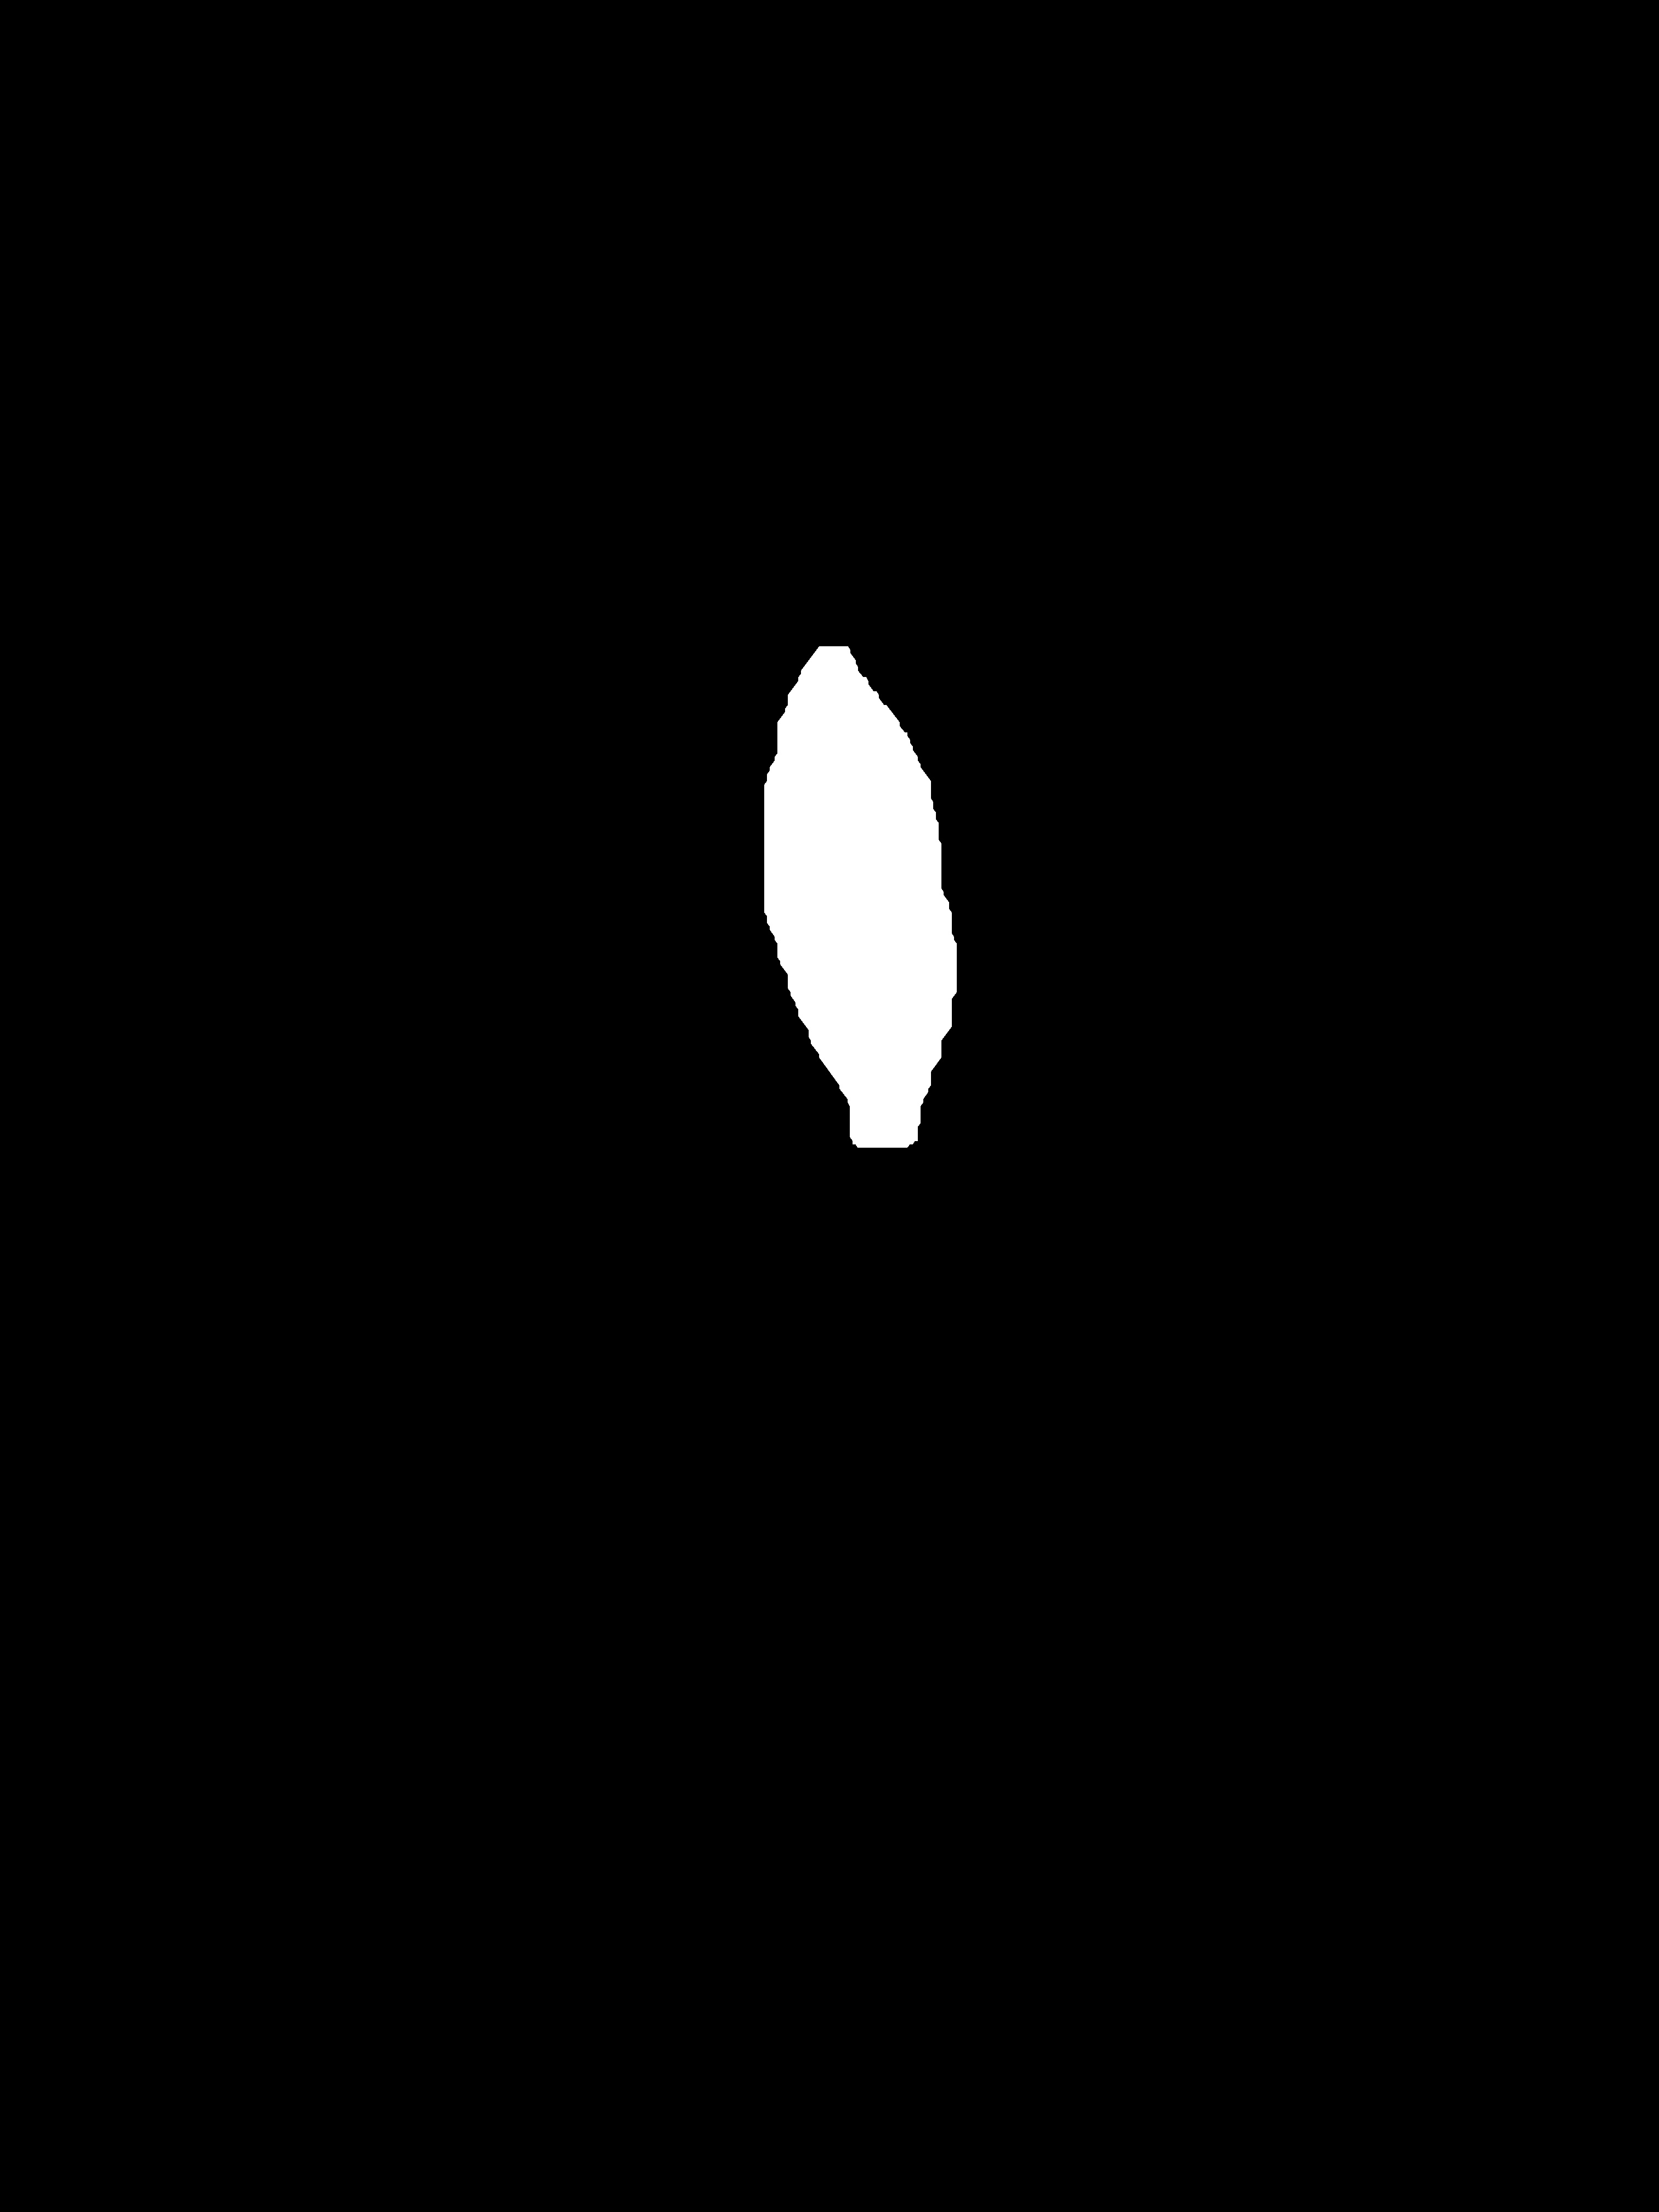
\includegraphics[width=\textwidth]{base_pesos_peixe/bd_mask/fish1799.jpg}
        \caption*{Máscara}
    \end{minipage}
    \hfill
    \begin{minipage}{0.31\textwidth}
        \centering
        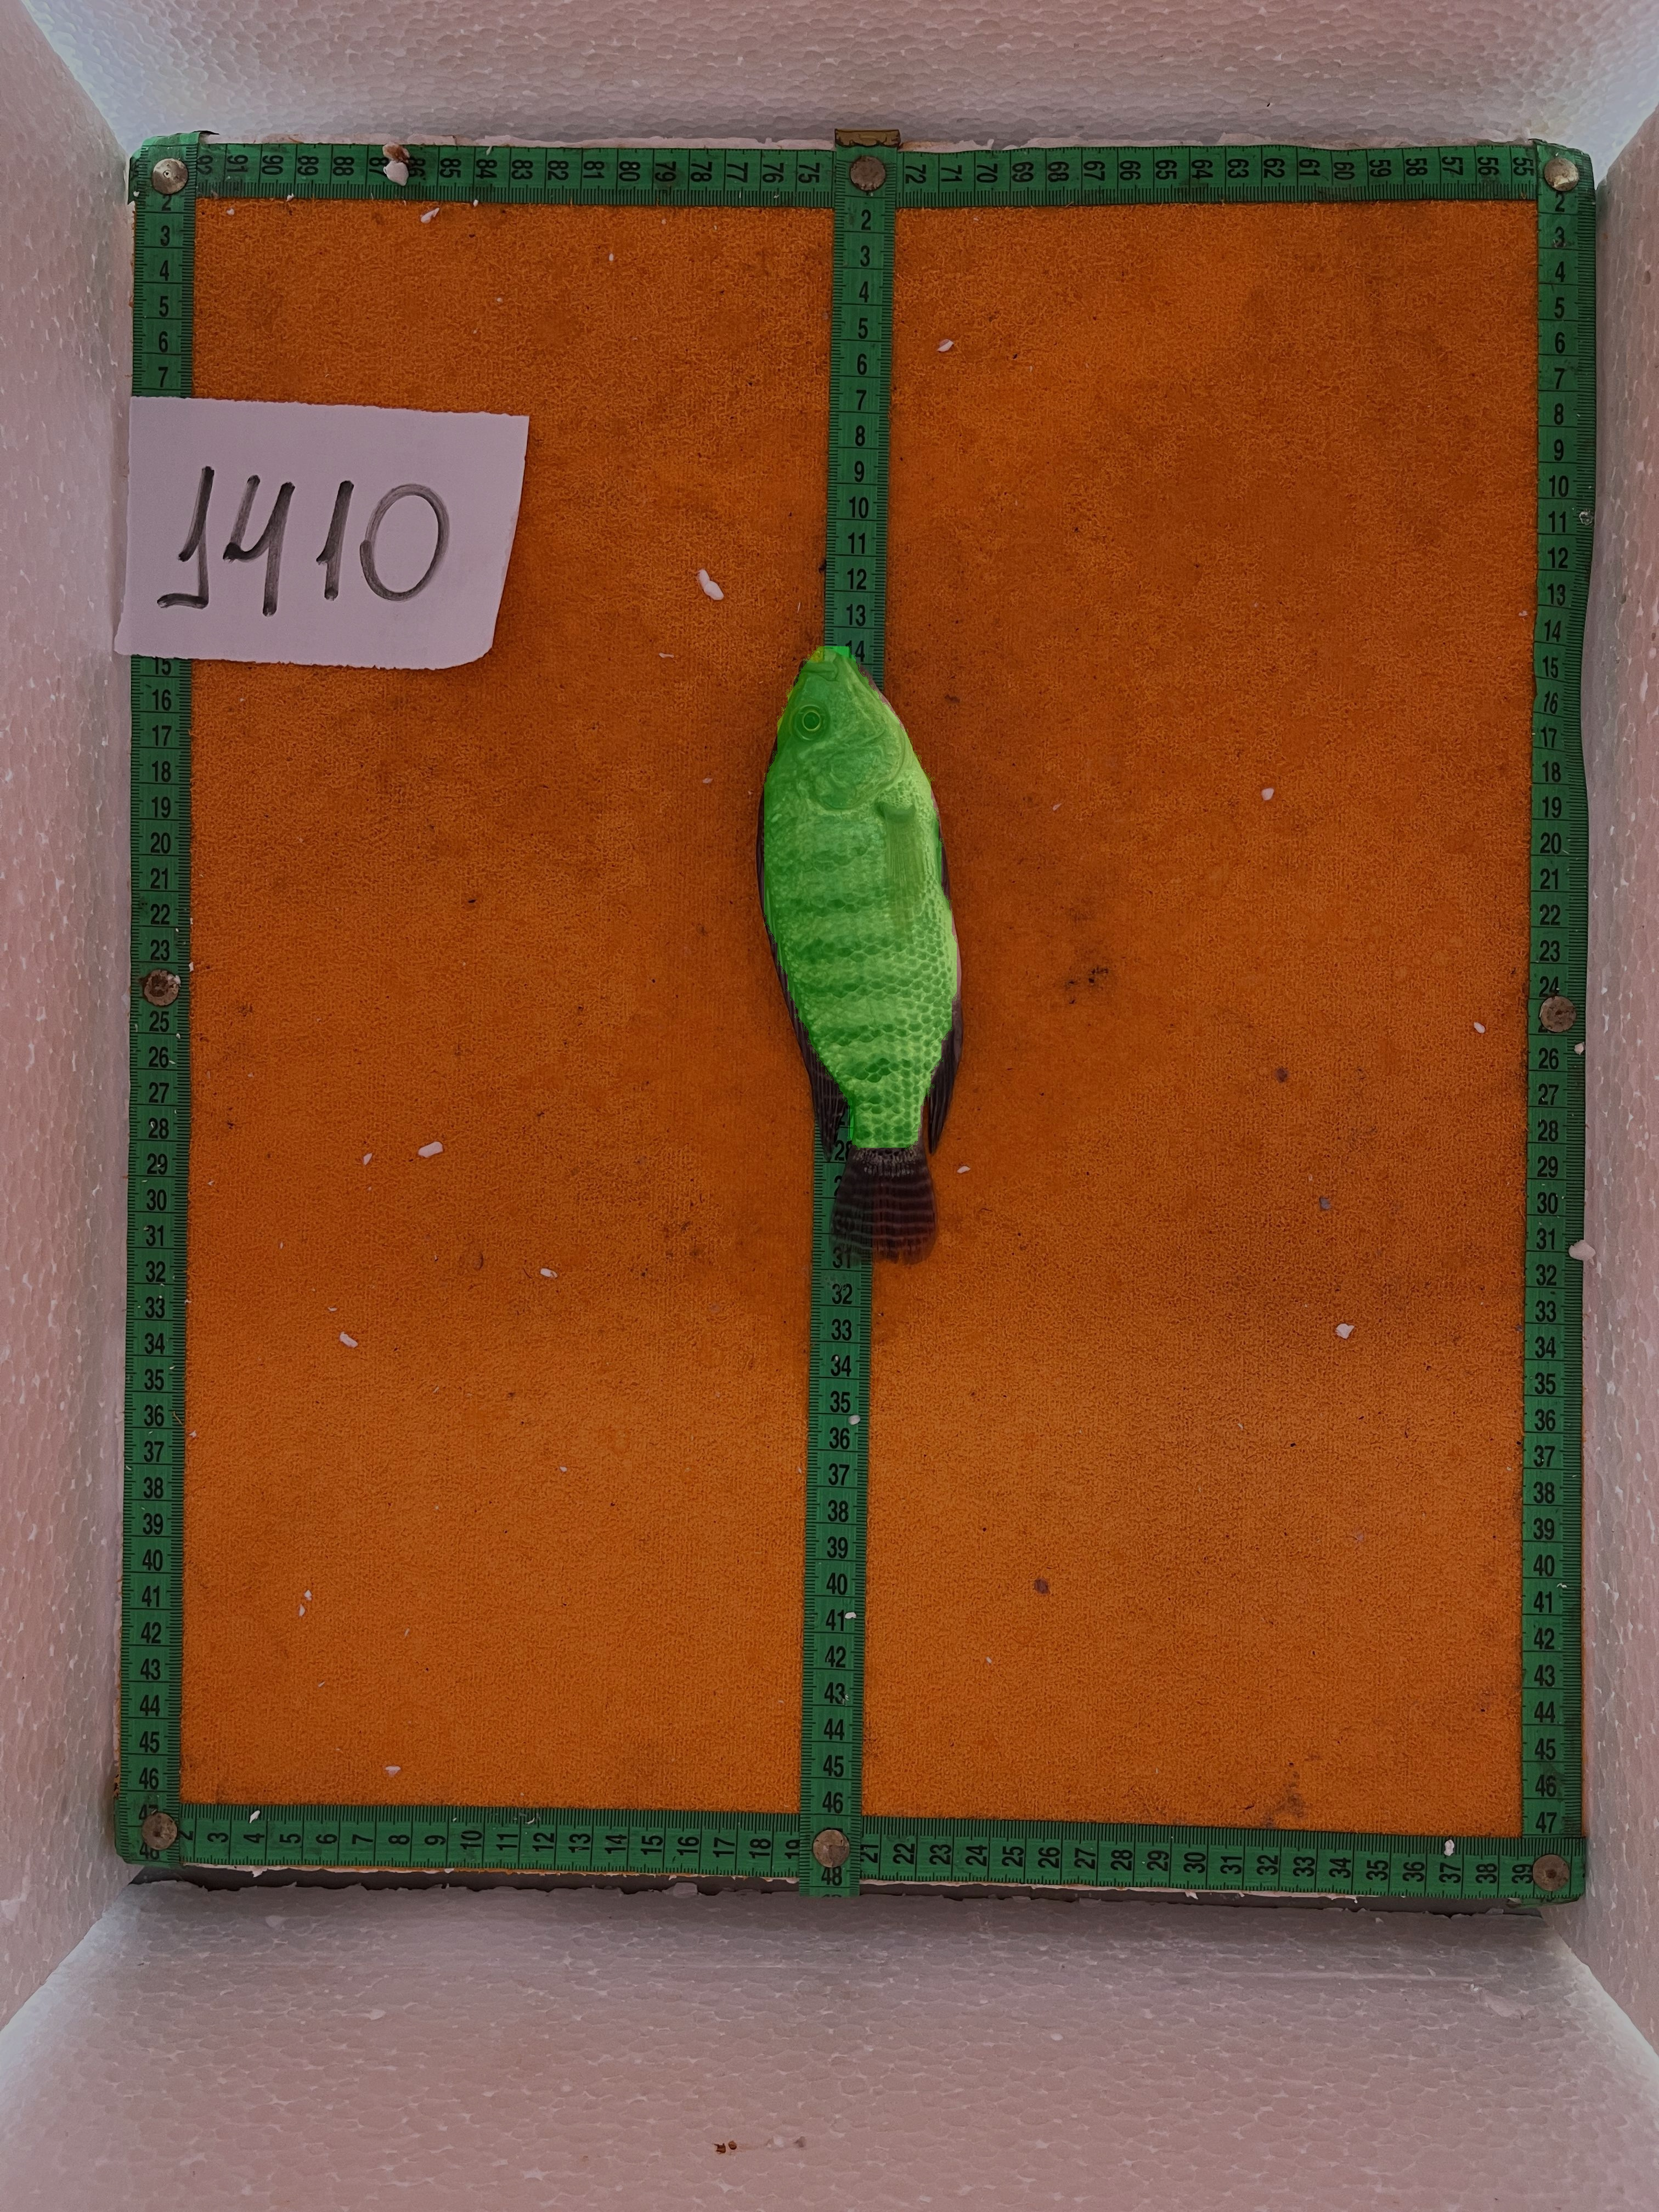
\includegraphics[width=\textwidth]{base_pesos_peixe/aplicacao_das_mascaras/fish1799.jpg}
        \caption*{Segmentada}
    \end{minipage}
    \caption{Processo de Segmentação de Imagem para Extração de Dados}
\end{figure}

\vspace{0.5cm}

\section*{Parte 1: Criação da Estrutura}
A tabela \texttt{peixes} armazenará atributos físicos extraídos de imagens. Execute o comando abaixo no \textit{Query Tool}:

\begin{lstlisting}[caption={Criação da tabela peixes}]
CREATE TABLE peixes (
    id TEXT,
    area INTEGER,
    perimetro DOUBLE PRECISION,
    ecentricidade DOUBLE PRECISION,
    maior_eixo DOUBLE PRECISION,
    menor_eixo DOUBLE PRECISION,
    peso INTEGER,
    classe INTEGER,
    compactacao DOUBLE PRECISION,
    rmm DOUBLE PRECISION,
    centroid_x DOUBLE PRECISION,
    centroid_y DOUBLE PRECISION
);
\end{lstlisting}

\vspace{0.5cm}

\section*{Parte 2: Importação de Dados (Processo ETL)}

Siga rigorosamente os passos abaixo para popular o banco com o arquivo \texttt{df\_final\_integrado.csv} através do pgAdmin 4.

\vspace{0.3cm}

\begin{block}{PASSO 1 --- Localizar a tabela}
No pgAdmin 4, navegue pela árvore de objetos:
\begin{verbatim}
Servers
 +-- unirv
      +-- Databases
           +-- postgres
                +-- Schemas
                     +-- public
                          +-- Tables
                               +-- peixes
\end{verbatim}
\end{block}

\begin{block}{PASSO 2 --- Abrir Importação}
Clique com o \textbf{botão direito} na tabela \texttt{peixes} e selecione a opção:
\begin{center}
    \textbf{Import/Export Data...}
\end{center}
\end{block}

\begin{block}{PASSO 3 --- Aba General}
Na aba \textit{General}, configure exatamente os seguintes campos:

\vspace{0.2cm}
\centering
\begin{tabular}{|l|l|}
\hline
\textbf{Campo} & \textbf{Valor} \\ \hline
Import/Export & Import \\ \hline
Filename & (selecione seu CSV) \\ \hline
Format & csv \\ \hline
Encoding & UTF8 \\ \hline
\end{tabular}
\vspace{0.2cm}

\flushleft
Clique no ícone de pasta e selecione o arquivo: \texttt{df\_final\_integrado.csv}
\end{block}

\begin{block}{PASSO 4 --- Aba Options (MAIS IMPORTANTE)}
Este é o ponto crítico para evitar erros de importação. Configure:

\vspace{0.2cm}
\centering
\begin{tabular}{|l|l|}
\hline
\textbf{Opção} & \textbf{Valor} \\ \hline
Header & YES \\ \hline
Delimiter & , \\ \hline
Quote & " \\ \hline
Escape & " \\ \hline
NULL String & (deixe vazio) \\ \hline
\end{tabular}
\end{block}

\vspace{0.5cm}

\section*{Parte 3: Análise Exploratória e Estatísticas}
Utilize funções de agregação para uma visão geral do dataset:

\subsection*{Estatística Descritiva}
\begin{lstlisting}
SELECT MAX(peso), MIN(peso), AVG(peso) FROM peixes;
\end{lstlisting}

\subsection*{Distribuição por Classe e Rankings}
\begin{lstlisting}
-- Contagem por classe
SELECT classe, COUNT(id) FROM peixes GROUP BY classe ORDER BY classe;

-- Top 10 peixes mais pesados
SELECT id, peso FROM peixes ORDER BY peso DESC LIMIT 10;
\end{lstlisting}

\vspace{0.5cm}

\section*{Parte 4: Filtragem Avançada e Qualidade}
Nesta etapa, aplicamos filtros específicos para segmentar os dados.

\subsection*{Identificação de Classes Únicas}
Para verificar quantas espécies ou grupos distintos foram catalogados:
\begin{lstlisting}
SELECT DISTINCT classe FROM peixes;
\end{lstlisting}

\subsection*{Filtros Combinados (WHERE)}
Isolando espécimes de grande porte de uma classe específica:
\begin{lstlisting}
-- Selecionar peixes pesados da classe 1
SELECT * FROM peixes 
WHERE peso > 1000 AND classe = 1;
\end{lstlisting}

\subsection*{Seleção por Faixa (BETWEEN)}
Útil para estudos de morfologia em intervalos específicos de ecentricidade:
\begin{lstlisting}
-- Selecionar peixes com ecentricidade entre 0.5 e 0.8
SELECT id, area 
FROM peixes 
WHERE ecentricidade BETWEEN 0.5 AND 0.8;
\end{lstlisting}

\vspace{1.0cm}

\begin{center}
    
\includegraphics[width=0.3\textwidth]{adriano_carvalho.jpg} \\
    \vspace{0.3cm}
    \textit{"Um cumprimento especial ao \textbf{Dr. Adriano Carvalho Costa} do Instituto Federal Goiano, pelo apoio e colaboração técnica neste projeto."}
\end{center}

\vspace{0.8cm}

\begin{center}
\textit{“Boa atividade! Att. Me. Prof. Sergio Souza Novak.”}
\end{center}

% =========================
\end{document}
% =========================